%
% Clase de codificador
% Análisis y diseño de programa tokenizador, reporte técnico.
%
% Proyecto Lovelace.
%

\subsection{Codificador de binario a ASCII}

Para evitar almacenar en formato binario las llaves generadas por el ejecutable
tokenizador, se implementó el codificador de binario a caracteres ASCII descrito
en el \gls{gl:rfc} 4648 \cite{DBLP:journals/rfc/rfc4648}. La idea es no guardar
una llave en su representación binaria, sino guardar solamente caracteres
imprimibles. Para esto, el codificador hace un mapeo de los bytes originales
(rango de 256 números) a bytes acortados, que se encuentren en un rango de 64,
32 o 16 números.

En la figura \ref{clases_codificador} se muestran la clase del codificador junto
con su relación con otras clases. Existe una enumeración para indicar las
distintas posibilidades de codificación. El codificador implementa a una función
con inverso, la cuál a su vez implementa a una función.

\begin{figure}
  \begin{center}
    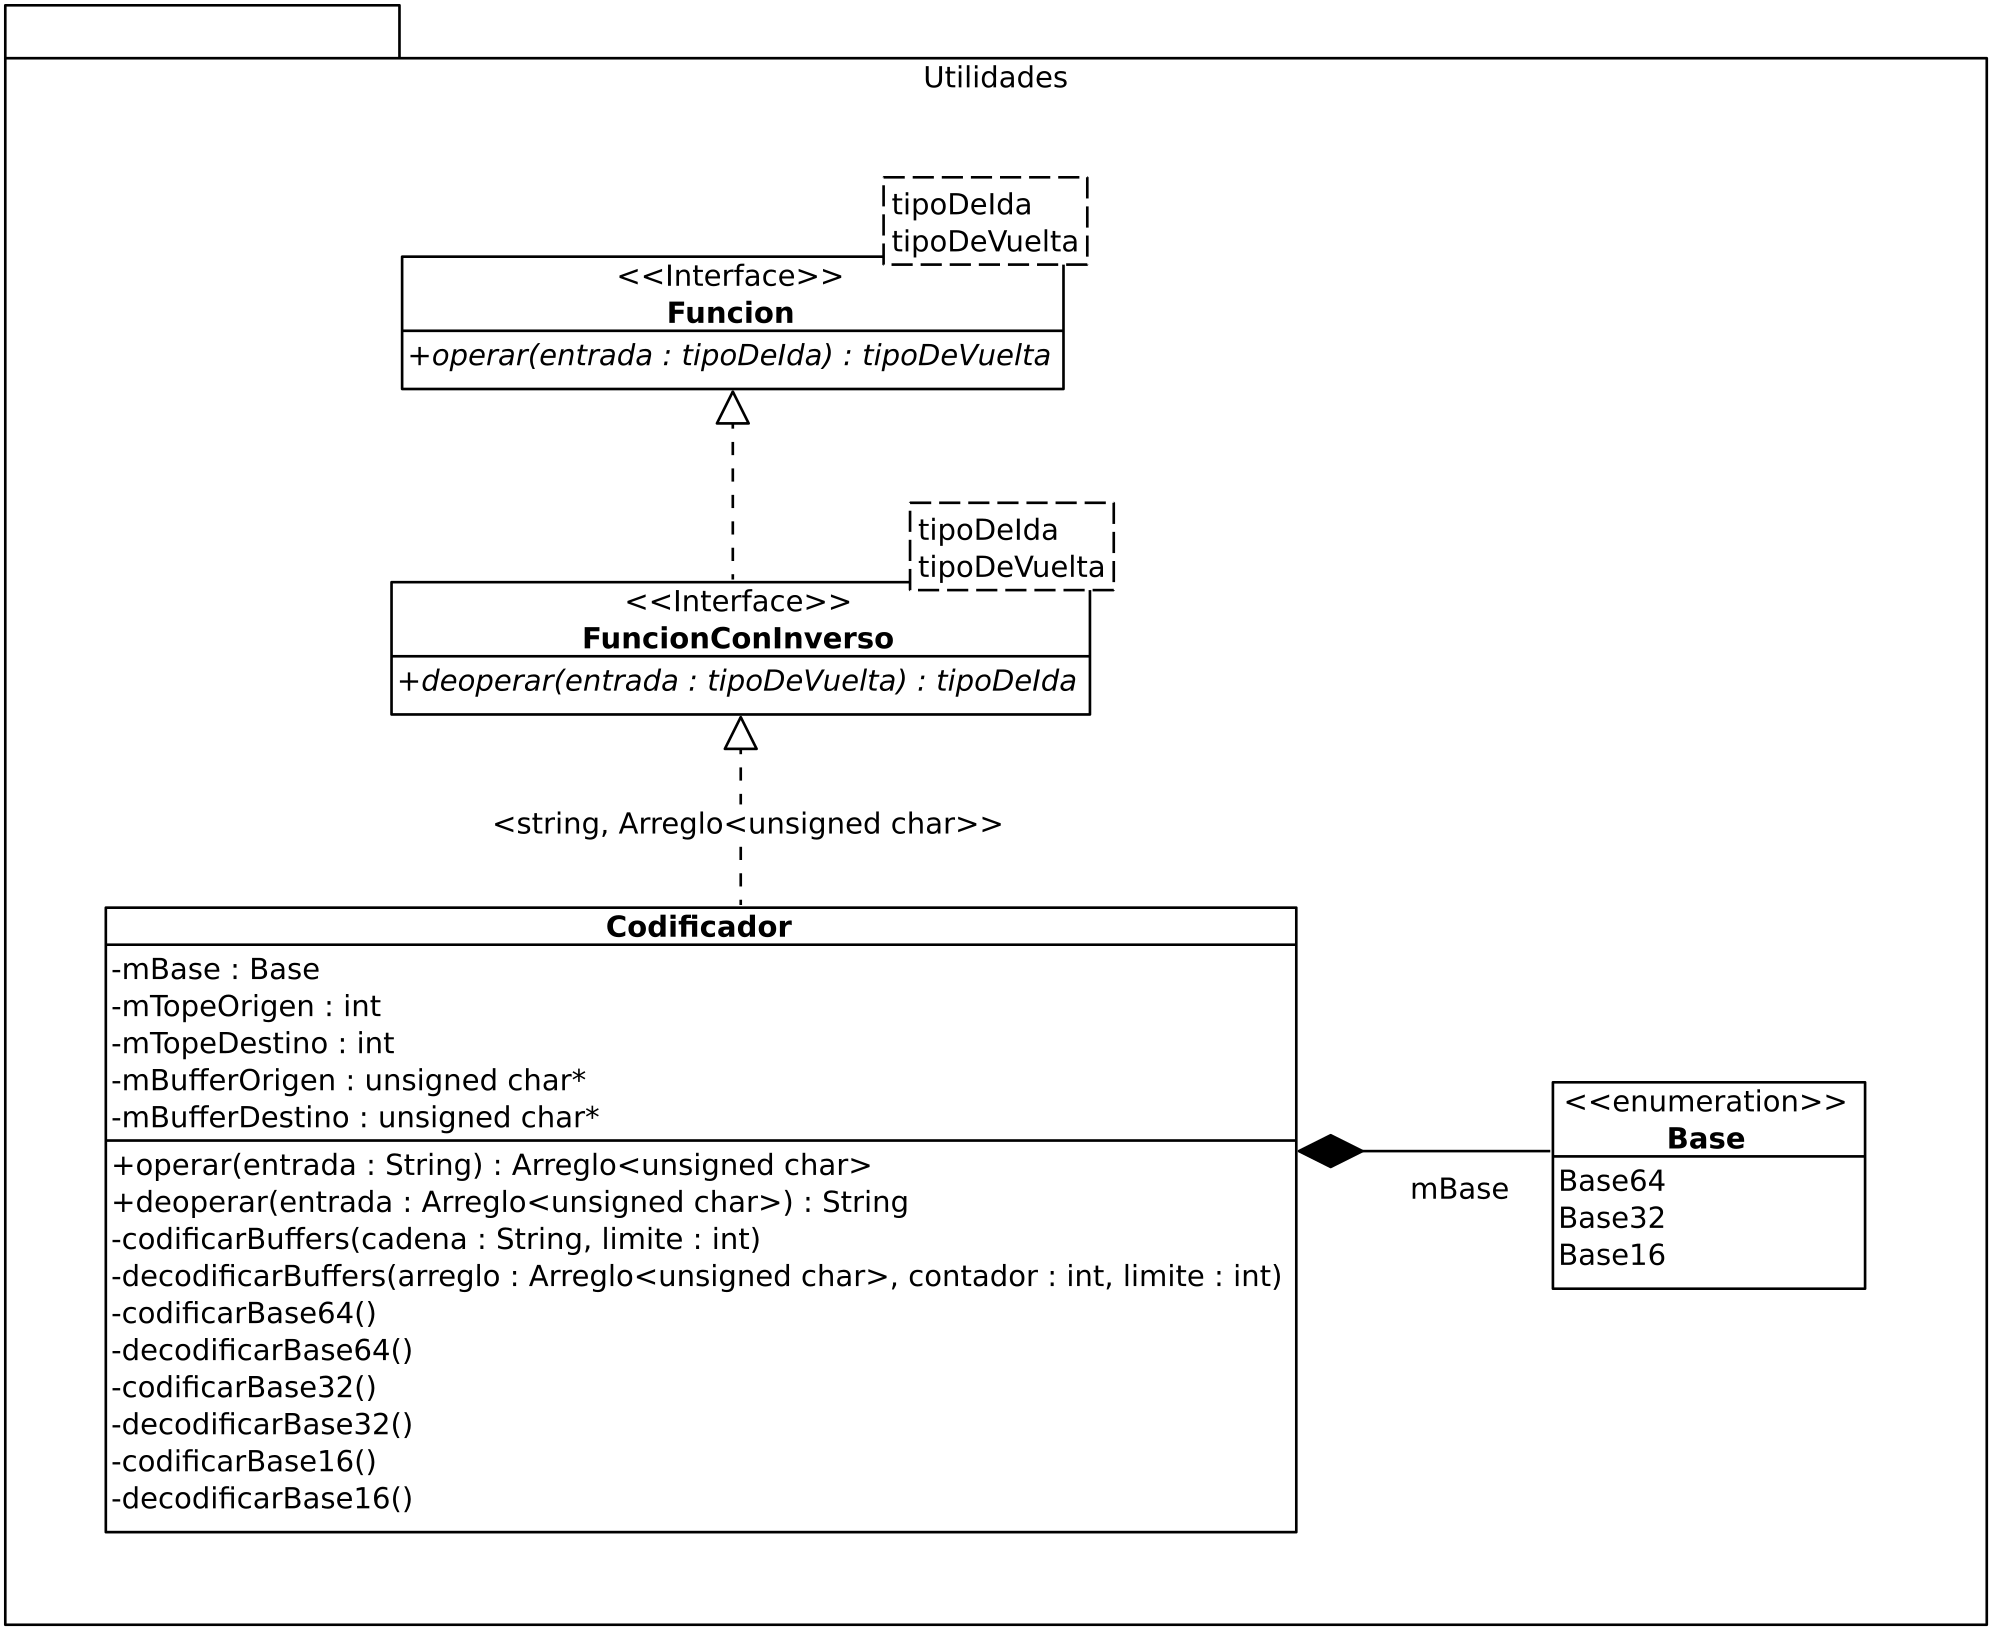
\includegraphics[width=0.7\linewidth]{diagramas/codificador.png}
    \caption{Clase de codificador.}
    \label{clases_codificador}
  \end{center}
\end{figure}
